\section{Framework}\label{sec:lexical}

We pose three research questions: (i) Does increasing CoT \length improve reasoning accuracy? (ii) Does increasing \Review improve reasoning accuracy? and (iii) What structural properties underlie the effects of \length and \Review? The first two questions are motivated by ongoing debates surrounding the S1 approach \citep{muennighoff2025s1}, while the third seeks to identify more fundamental structural drivers of reasoning performance. In this section, we will outline the framework and define these metrics.

\subsection{Setup}

\paragraph{Dataset} \quad We leverage the HARP dataset \citep{yue2024harp}, which is centered on mathematical reasoning, and the GPQA-Diamond dataset \citep{rein2024gpqa}, which covers scientific reasoning. Both datasets have human-labeled difficulty levels, allowing us to examine patterns across different difficulty strata. The HARP dataset comprises 5,409 math questions sourced from U.S. national math competitions. To reduce computational load, we subsample 50 questions from each of the 6 difficulty levels. We take all 198 questions from GPQA-Diamond.

\paragraph{Models} \quad We analyze different model family and different model sizes, including both dense models and mixture of expert models.

\textit{Proprietary models with CoT access}:  Claude 3.7 Sonnet Thinking, Grok 3 mini.

\textit{Open Sourced Families}: Deepseek R1 (20250120), Deepseek Distill Qwen 32B (Deepseek 32B), Deepseek Distill Qwen 7B (Deepseek 7B), Qwen 3 235B, Qwen 3 32B, Qwen 3 8B, GPT oss 120B, GPT oss 20B.

For each question, we generate 16 reasoning traces to ensure that we have enough observations. This allows our analysis to condition on the question to rule out any question-related confounding factors. In total, we analyze 4,800 math reasoning traces and around 3,200 general science reasoning traces for each model.

\subsection{Metrics}

To fairly compare between different models when the tokenizer is different, the following metrics are defined at the character level. 

\Length. We define the CoT \Length in characters.

\Review. We measure \Review behavoirs with an LLM-as-a-judge procedure. Each reasoning trace is segmented into chunks using keyword-based heuristics (full list in Table \ref{app-tab1:keywords}). We then prompt the Llama 4 Maverick model~\citep{meta2025llama} to label each chunk as \progress or \review; the model receives the current chunk together with the preceding five and the subsequent five chunks to provide activity context. We use the following semantics:


\begin{description}
\item \textit{progress}: advances the active reasoning frontier, producing information that later steps rely on.
\item \textit{review}: reads, checks, restates, deletes, or rewinds existing material without advancing the frontier.
\end{description}

% \begin{description}
%     \item[\texttt{progress}:] A step that extends the active reasoning frontier, producing information the solver will rely on later.
%     \item[\texttt{review}:] A step that reads, checks, restates, deletes, or rewinds existing material without advancing the frontier.
% \end{description}

% Specifically, Let $c_i$ denote the $i$-th chunk, and $s_j$ denote the $j$-th character. When calling the Maverick model, we provide the current chunk $c_i$ along with the preceding 5 chunks and the subsequent 5 chunks to offer context on the model's activity. The full prompt used for the model can be found in the appendix.

%The authors further hand-label a validation set under these definitions; 
To measure labeling accuracy, we annotate a validation set in-house. We find that Maverick achieves ~90\% agreement with human labels, with minimal instances of {\textit{progress}} being mistaken for {\textit{review}}. Detailed error analysis is presented in Appendix \ref{appendix:alignment_review}.

% Metric definition
With the annotation, we calculate the character-level \rr for each reasoning trace: let $s_{t,j}$ denotes the $j$-th character in trace $t$ and $N_t$ its total number of characters,
\[
\rr_t \;=\; \frac{1}{N_t}\sum_{j=1}^{N_t} {1}\!\left[s_{t,j}\ \text{lies in a }\Review\ \text{chunk}\right].
\]

% With the annotation, we calculate the character level Review Ratio for each reasoning trace:

% \begin{description}
%     \item[\textbf{Review Ratio}] 
%     $$
% RR_i = \frac{1}{N_i} \sum_{j=1}^{N_i} (s_j \text{ is } \review), \quad \text{where } N_i \text{ is the number of characters in the } i \text{-th trace.}
% $$
% \end{description}

\paragraph{Reasoning Graph} A CoT naturally unfolds step by step, with steps varying in length and purpose. \Length and \rr are token-level (character-level) measures that can conflate verbosity with process quality. We further extract a reasoning graph for each CoT to probe structural properties.

Specifically, we prompt Claude 3.7 sonnet with thinking disabled to convert each CoT into Graphviz format \citep{gansner2009drawing}. Modern LLMs produce valid Graphviz codes with high fidelity, likely due to lots of Graphviz data used during pretraining. Figure~\ref{fig:data_visualization} visualizes one example: we extract a faithful reasoning graph that generally matches the steps in the natural-language trace. Our extraction procedure is simple, yet yields sufficiently accurate graphs, avoiding the complex prompting or embedding pipelines of \citet{jiang2025makes, minegishi2025topology}. The Claude-produced graphs compiled without error in 100\% of cases. Full extraction details and the complete list of graph metrics are provided in Appendix \ref{appendix:graph}.

Among graph metrics, we highlight one candidate as a potential structural driver of \Length and \rr:

\failedstep, the fraction of reasoning nodes in the graph that are marked as failed/abandoned:
$$
\fsf = \frac{\text{\# failed nodes}}{\text{\# all nodes}}.
$$
During extraction, we ask the model to color-code nodes as successful or failed attempts\footnote{We emphasize that the “failed attempt” label is local to the reasoning trajectory (e.g., an abandoned branch), not a judgment of step correctness. A CoT may yield an incorrect final answer while every step is labeled “successful”—even when Claude is able to correctly judges the final answer as wrong.}. This labeling enables a direct computation of the failed-step fraction. 

In Figure~\ref{fig:data_visualization}, we provide an example CoT with the chunks and annotations of \textit{progress} and \textit{review}, and the extracted reasoning graph.

Beyond these core metrics, we also evaluate additional graph-based measures (Appendix \ref{appendix:graph}) and stylistic features including motivation levels (Appendix \ref{append:other metrics}), and progressiveness similar to \citep{wu2025knowledge} (Appendix \ref{append:further}). See the corresponding appendices for detailed definitions.

% it is essential to model this variable within our system and generate a sufficient number of reasoning traces for each question to isolate the effect of the question itself. We have decided to generate 16 responses per question, using four different temperature settings: 0.3, 0.6, 0.8, and 1.0. This ensures adequate coverage of reasoning patterns.

% these metrics are sufficient? We note that the significance is not a global trend: it is not consistent across all models. Furthermore, both metrics are token-level (character-level) measures that can conflate verbosity with process quality. 

% However, a CoT naturally unfolds step by step, with steps varying in length and purpose. We therefore hypothesize that \Length and \rr are surface proxies for deeper structural properties of the underlying reasoning. To test this, we extract a reasoning graph for each CoT and evaluate graph-level metrics in this section.








\begin{figure}[tb]
    \centering
    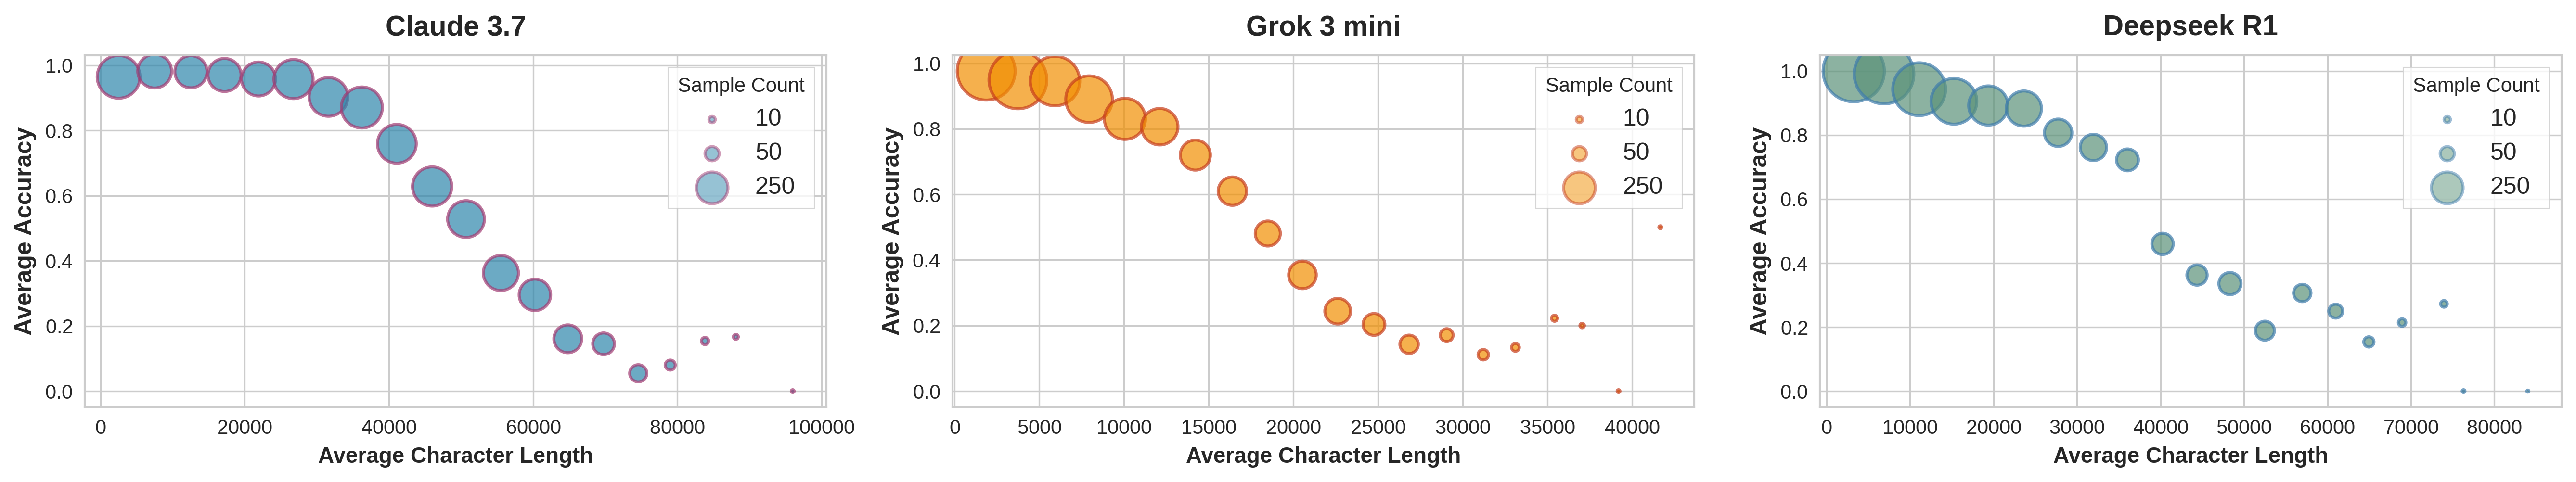
\includegraphics[width=\linewidth]{fig_tmp/level_correlation_length.png}
    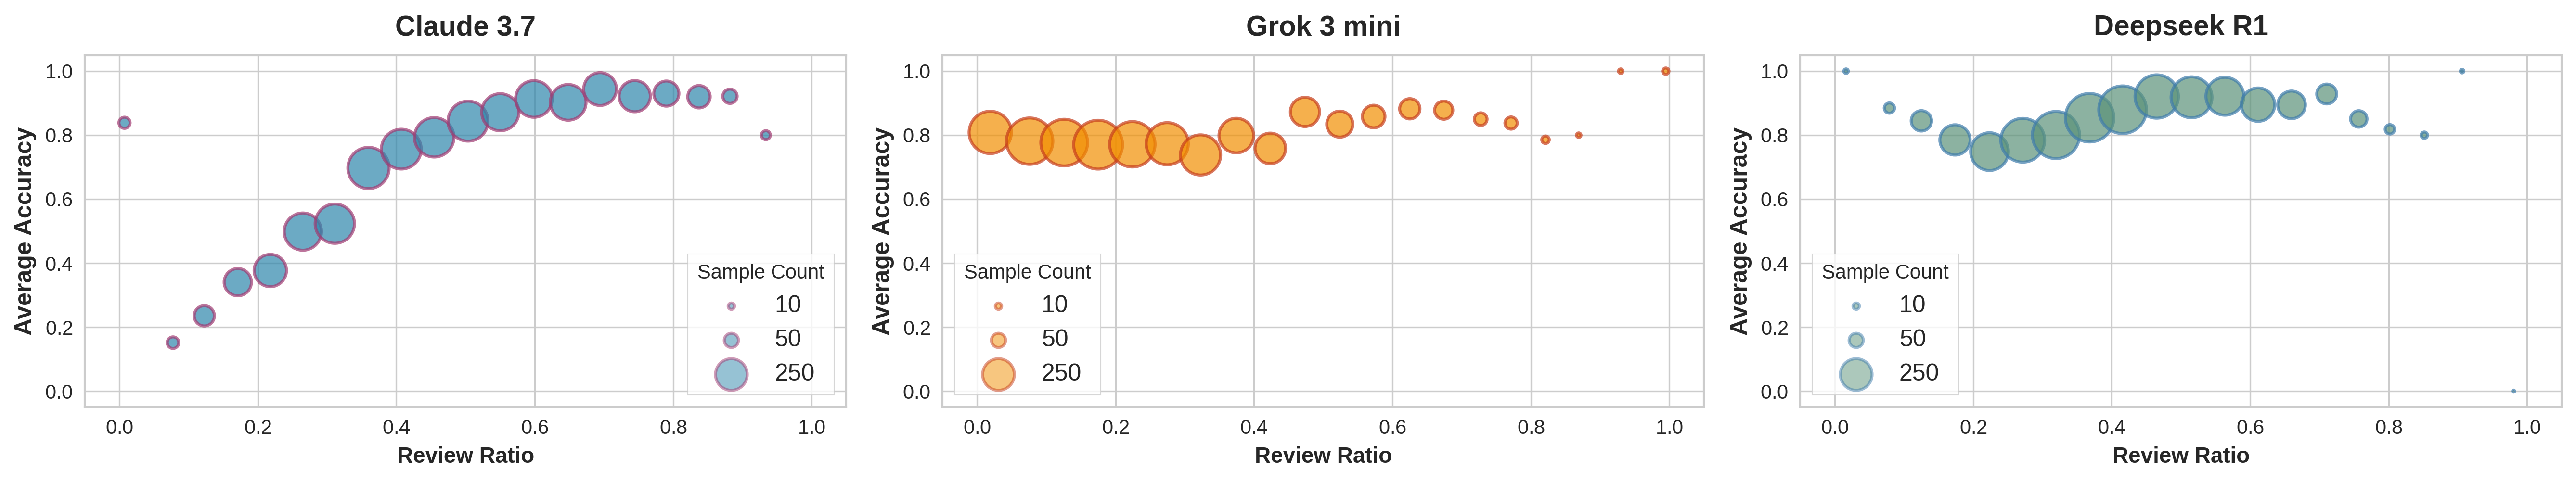
\includegraphics[width=\linewidth]{fig_tmp/level_correlation_review_ratio.png}
    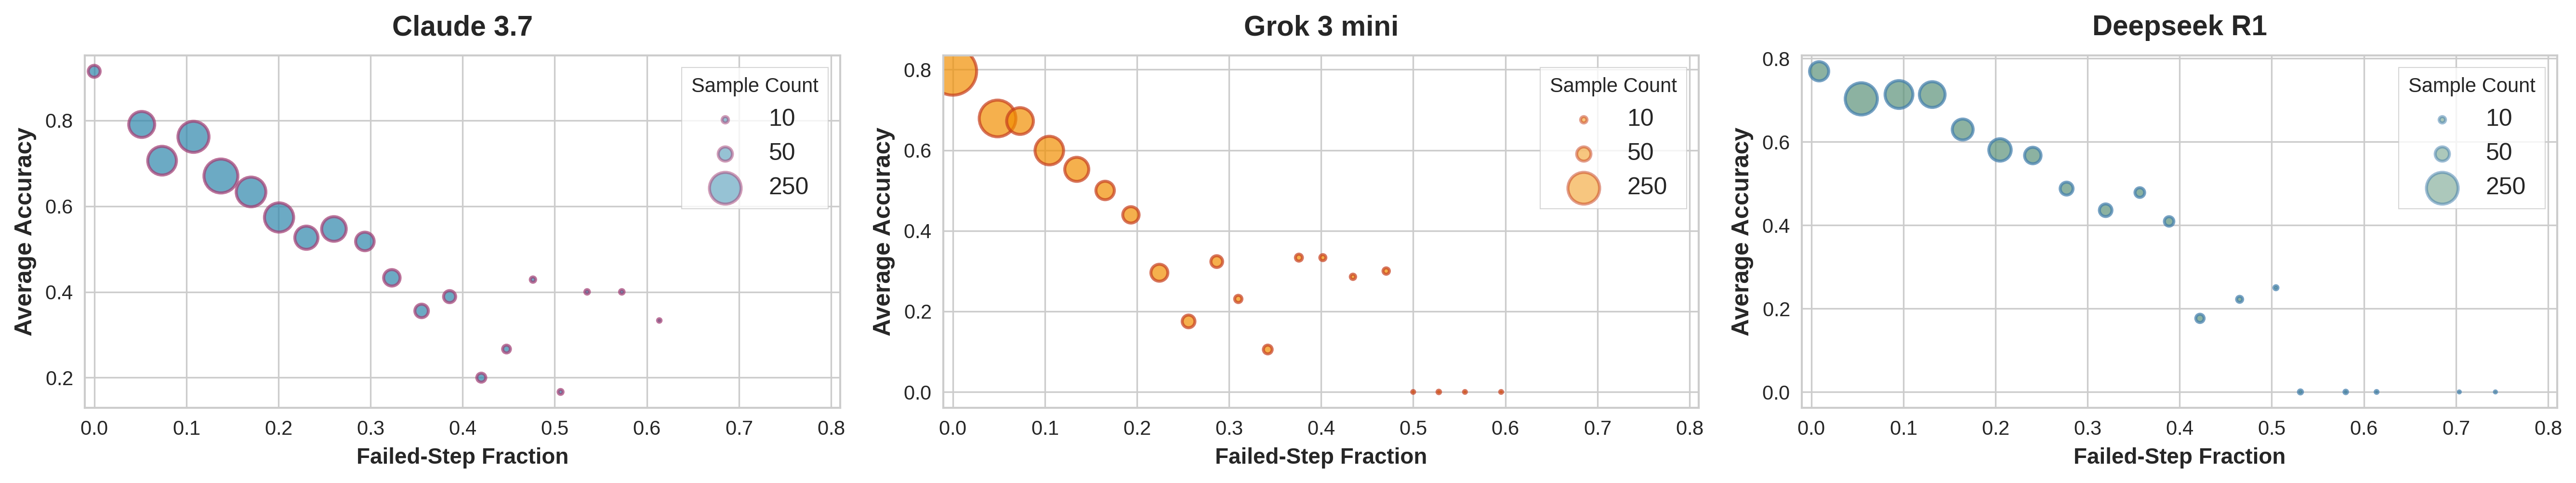
\includegraphics[width=\linewidth]{fig_tmp/level_correlation_fsf.png}
    \caption{Distribution of the three metrics—\Length, \rr, and \failedstep and their correlation with accuracy. All measured on CoTs generated for the Level 6 (hardest) subset of the HARP dataset. All three metrics exhibit correlation, with \fsf the strongest.}
    \label{fig:level_correlation_length}
\end{figure}

% \subsection{Conditional Correlation}

\begin{figure}[tb]
    \centering
    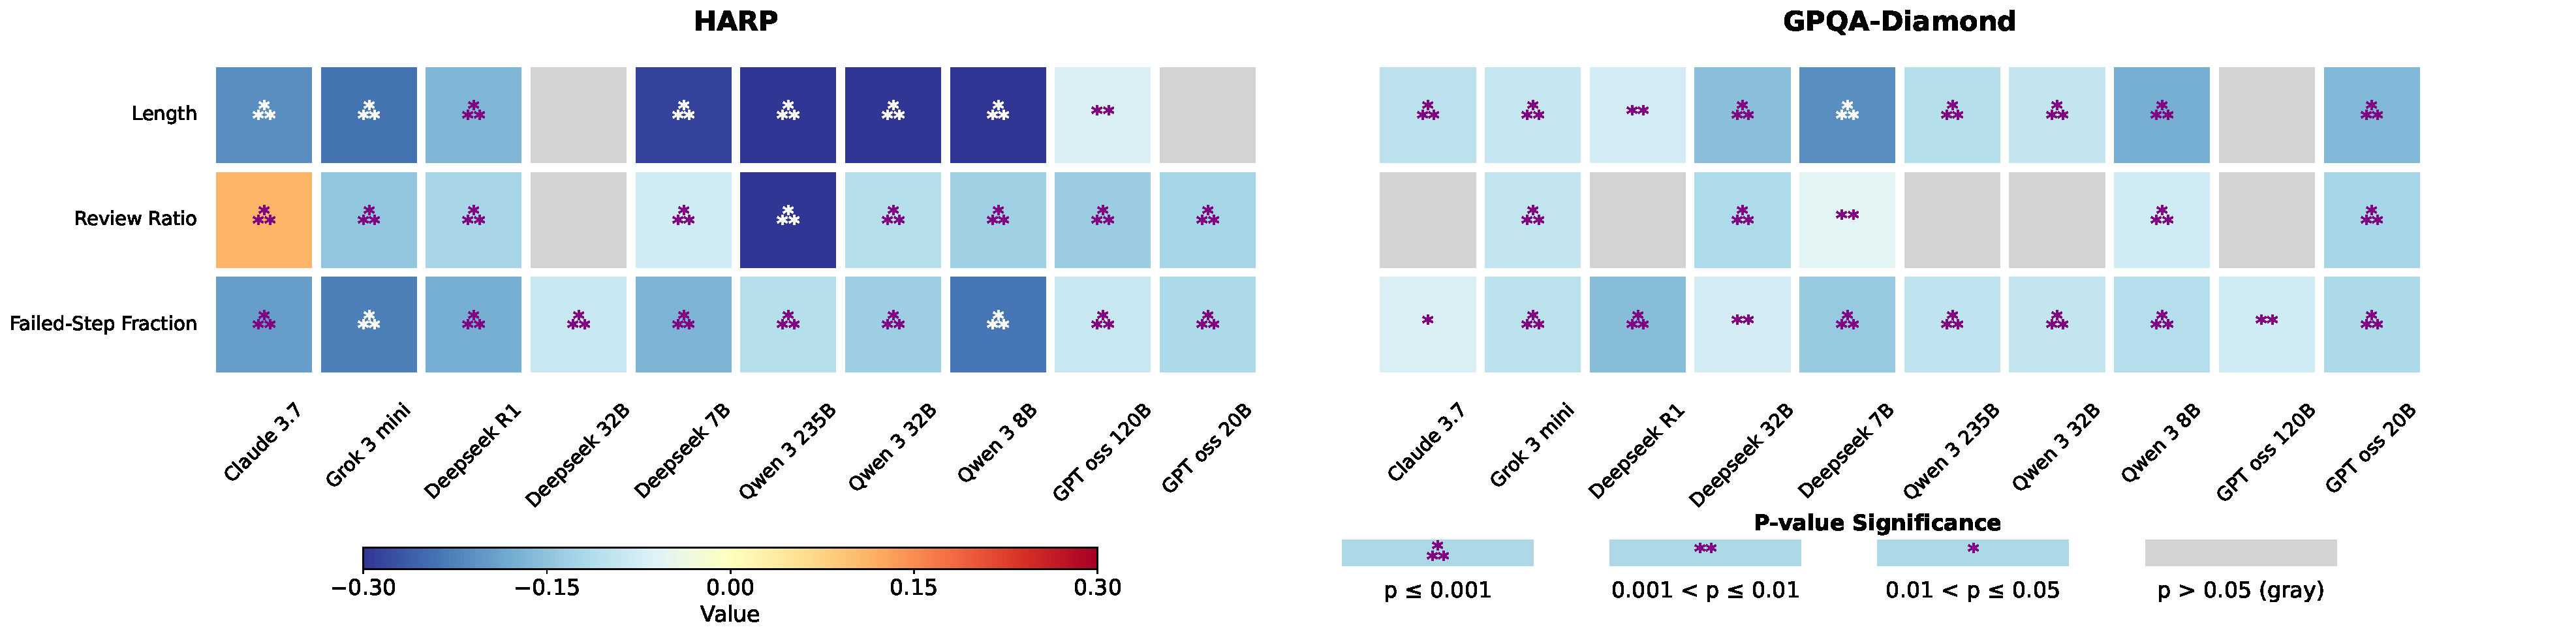
\includegraphics[width=\linewidth]{final_figs/correlation_all.pdf}
    \caption{Conditional correlations computed on the full dataset. Correlations are shown with a color scale; non-significant cells (\(p>0.05\)) are grayed out, and * denotes statistical significance (see the legend). We color * white or purple for visualization only. More colored cells indicate broader prevalence of correlation; darker colors denote stronger correlations. When controlling for question-level confounders, all three metrics correlate with accuracy, with \fsf significant across all models and both datasets.}
    \label{fig:correlation_harp_all_3}
\end{figure}





% In addition, we fit a Bayesian Generalized Linear Mixed-effects Model (GLMM) for correctness as a function of each metric with question-level random effects, and the coefficient shows the correlation strength. Full GLMM results are in Appendix \ref{append:glmm}. Among all results, we see strong alignment with conditional correlation results: all the significant coefficients in GLMM align with the significant correlation in conditional correlation test. It provides a second line of evidence. 

% \textcolor{red}{please add section number?? Also can we please add one line summary of these results.}.

% \subsection{Conditional Correlation}

% \textit{In conclusion, shorter length and lower review ratio generally correlate with higher accuracy, with effects in math more pronounced on harder questions.}

\section{Correlation Analysis}\label{sec:graphical}

We now present our results, beginning with general distribution visualizations, followed by conditional correlation analyses that control for confounding factors.

\subsection{Metric Distributions}

We first visualize the distributions of \Length, \rr, and \fsf with accuracy in Figure \ref{fig:level_correlation_length} using the HARP Level-6 set (the hardest split). In general, across all three models, shorter CoTs are associated with higher accuracy. For \rr, Claude 3.7 shows a positive trend: higher \rr brings higher accuracy, while the other two models are mixed. For \fsf, less \fsf are correlated with higher accuracy, with an approximately linear relationship. However, drawing broad conclusions from raw correlations is risky because of confounding factors. For example, harder questions or specific domains (e.g., algebra) may require longer CoTs and more \Review behavior, while also having lower accuracy, which can induce spurious correlations.

To mitigate these confounders, we generate 16 CoTs per question and run a conditional correlation test that conditions on the question level. Specifically, for each metric, we subtract the question-level mean from each of the CoT’s value (i.e., include question fixed effects) and then correlate these residualized values with residualized correctness across all data. This controls for question-level heterogeneity and yields reliable estimates. In this correlation analysis, we filter out questions where all generations are correct or all are incorrect, as they provide no signal.

In addition, we fit a Bayesian generalized linear mixed-effects model (GLMM) for correctness as a function of each metric, with random intercepts at the question level. The coefficient for each metric captures the direction and magnitude of association. Full model specification and results are provided in Appendix~\ref{append:glmm}. The GLMM results align closely with the conditional-correlation analysis: whenever the conditional correlation is significant, the corresponding GLMM coefficient is significant with the same sign. This concordance provides a second line of evidence.

\subsection{Conditional Correlation Analysis}\label{sec:graph-result}


\paragraph{Overall Conditional Correlations} We report conditional correlation results in Figure \ref{fig:correlation_harp_all_3} for all the CoTs on HARP and GPQA-Diamond. Cell color encodes the correlation’s sign and magnitude; p value significance is indicated by stars (*** \(p\le0.001\), ** \(0.001< p\le0.01\), * \(0.01< p\le0.05\)). Cells with p > 0.05 are grayed out, denoting lack of statistical significance. Therefore, more colored cells indicate broader prevalence of correlation; darker colors denote stronger correlations.

For \Length, we observe a consistent negative correlation across both datasets and most models at the CoT level: shorter CoTs correlate with higher accuracy. For \rr, most models similarly exhibit significant negative correlations, with lower \rr associated with higher accuracy. Claude 3.7 on math reasoning presents a notable exception, showing the opposite trend as illustrated in Figure \ref{fig:level_correlation_length}. These findings provide clarity on the S1 debate and support recent observations in \citep{wu2025more, hassid2025don}.

For \failedstep, we find that \fsf correlates significantly with accuracy across every model in both math and scientific reasoning tasks, yielding more consistent correlations than either \Length or \rr. The pattern is robust: lower \fsf consistently correlates with higher accuracy -- even for Claude, which uniquely benefits from higher \rr unlike other models. All these patterns support \fsf as the intrinsic driver behind \Length and \rr effects. 

\paragraph{Conditional Correlations by Difficulty Level} Different questions may require different solution strategies. The human-labeled difficulty level reflects how complex a question is by human standards. We therefore compute conditional correlations within each difficulty level to test whether the correlation hold across difficulty strata. Results are shown in Figure \ref{fig:correlation_loxical_1}. We omit Level 1 in HARP and the Post-graduate level in GPQA-Diamond because the correlation test in these strata includes fewer than 100 CoTs. 

We observe distinct patterns when stratifying by question difficulty across both datasets. On HARP, correlations are most consistently significant on harder items (levels 4, 5, and 6) for all three metrics. This concentration is intuitive: for easier questions, models can succeed along multiple trajectories, weakening metric-accuracy correlations. Correspondingly, on easier questions, we see mixed patterns, with some Deepseek-class models occasionally benefiting from higher \rr and longer \Length. Within GPQA, we find consistent patterns across the Hard Undergraduate and Hard Graduate splits. \Length remains a prominent predictor, while \rr shows less consistent significance within difficulty bands, aligning with the weak \rr effects on GPQA shown in Figure \ref{fig:level_correlation_length}. Notably, while Claude 3.7 shows no significant correlation across all GPQA data, it does exhibit correlation within the Hard Graduate split, demonstrating that difficulty-specific patterns can be masked in aggregate analyses.

Across both datasets, \fsf demonstrates the strongest and most consistent performance. When significant correlations emerge, \fsf exhibits consistent negative correlations across all models and difficulty levels, with more significant correlations than either \Length or \rr. This further supports \fsf as the key structural metric.



\begin{figure}[tb]
    \centering
    % \includegraphics[width=\linewidth]{fig_tmp_2/harp_level_correlation.png}
    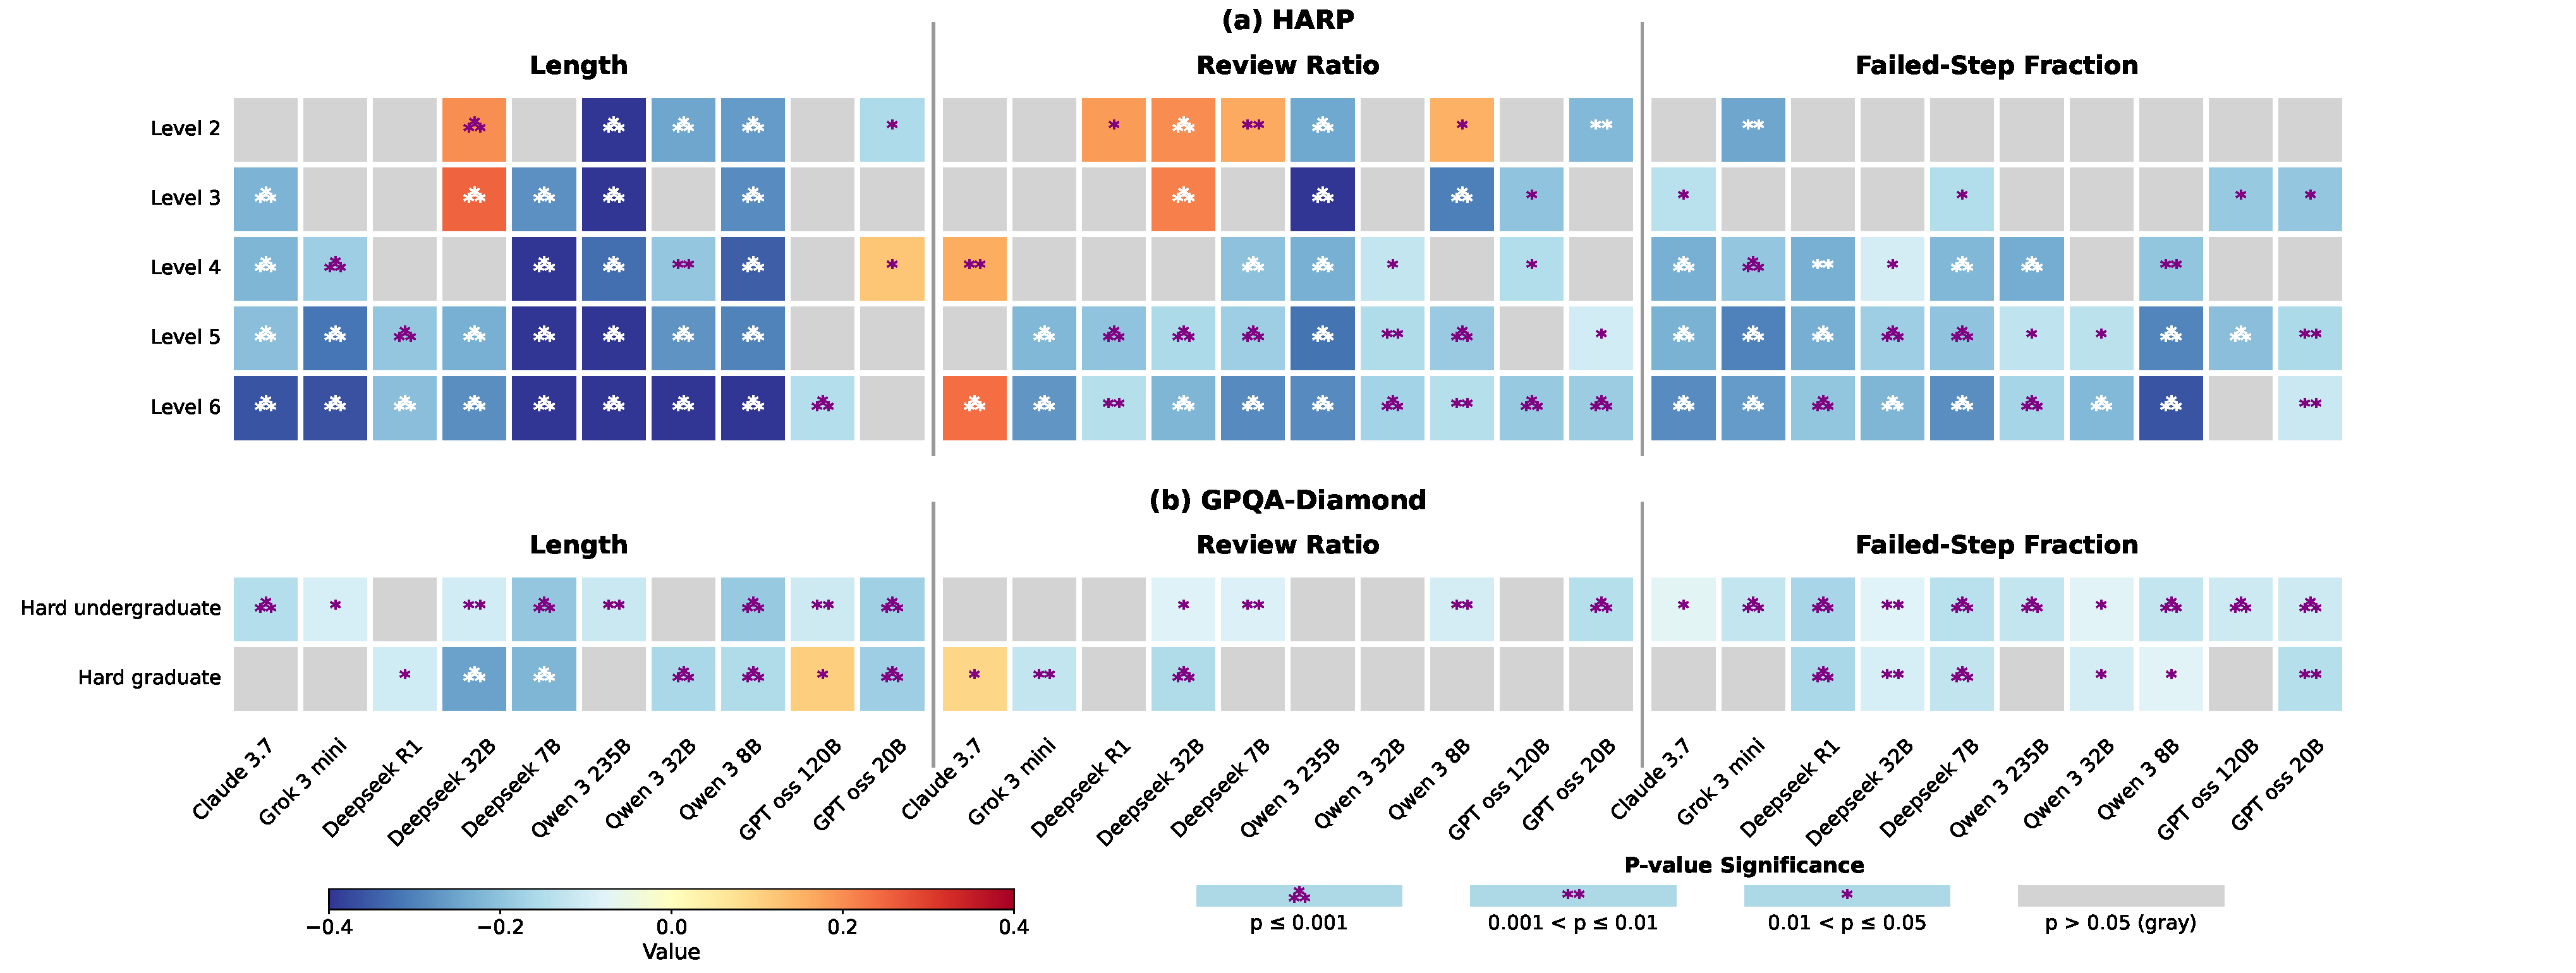
\includegraphics[width=1.08\linewidth]{final_figs/correlation_levels_combined.pdf}
    \caption{Conditional correlation by human-labeled difficulty level for generated CoTs. Top: HARP; bottom: GPQA-Diamond. Similarly, correlations are shown with a color scale; non-significant cells (\(p>0.05\)) are grayed out, and * denotes statistical significance (see the legend). We color * white or purple for visualization only. In math reasoning, correlations are stronger for harder questions.}
    \label{fig:correlation_loxical_1}
\end{figure}

In summary, we highlight the following observation:

\begin{tcolorbox}[colback=metablue!7]
Across CoTs for the same question, shorter \Length, lower \rr, and lower \fsf all generally correlate with higher accuracy, with more pronounced effects on harder math questions. \failedstep stands out as the strongest and most consistent predictor.
\end{tcolorbox}

Beyond \fsf, we evaluate correlations for additional graph-based metrics, which show consistently weaker effects than \fsf and are mostly significant only on math reasoning tasks (full results in Appendix~\ref{appendix:graph}). We also examine stylistic features including motivation levels, review positions, and progressiveness entropy (Appendices~\ref{append:other metrics} and \ref{append:further}). These analyses reveal that models exhibit distinct generation styles, but these stylistic features fail to correlate consistently with accuracy across models. These model-dependent behaviors would introduce bias when comparing metrics across models, reinforcing our methodological approach: estimating correlations within each model, then identifying patterns that replicate across models.


% The difference between Review Ratio and Failed-Step Fraction is that, Failed-Step Fraction characterize semantical step level ratio, and typically does not contain verifications; review ratio counts lexical character level ratio, and include all the verification.

% \todo{Add one bar chart for the top-1 score. Remove the curve for the judge.}

% \begin{figure}[tb]
%     \centering
%     \includegraphics[width=0.45\linewidth]{fig_tmp/correlation_fsf_1.png}
%     \includegraphics[width=0.45\linewidth]{fig_tmp/correlation_fsf_2.png}
%     \caption{Correlation results for Failed-Step Fraction. HARP dataset. Top: human labeled difficulty level; Bottom: model dependent difficulty level.}
%     \label{fig:correlation_fsf_1}
% \end{figure}

% \begin{figure}[tb]
%     \centering
%     \includegraphics[width=\linewidth]{fig_tmp/pass_1/correlation_mmlu_loxical_2.png}
%     \caption{Correlation results for Length, Review Ratio, and Review Fraction. MMLU pro dataset. model dependent difficulty level.}
%     \label{fig:correlation_mmlu_loxical_2}
% \end{figure}

% \begin{figure}[tb]
%     \centering
%     \includegraphics[width=0.45\linewidth]{fig_tmp/pass_1/correlation_mmlu_fsf_2.png}
%     \caption{Correlation results for Failed-Step Fraction. MMLU pro dataset. model dependent difficulty level.}
%     \label{fig:correlation_mmlu_fsf_2}
% \end{figure}


